
\chapter{作曲に関する経緯}

\section{背景}\label{sec: background}

%19世紀における交響曲の位置づけ
Beethoven以後のドイツ/オーストリアの作曲家にとって, 交響曲はBeethovenの重圧を感じずにはいられない分野であった.

%新しい道

%作曲に取り掛かる以前の話


\section{作曲過程}\label{sec: process}

作品68と後にBrahms自身によって附番されたこのハ短調の交響曲は, 少なくとも1862年の夏には着想されており, ある程度作曲が進んでいた.
Brahmsの友人である作曲家のAlbert Dietrichが1862年6月にバート・クロイツナハ近郊のミュンスター・アム・シュタインに滞在中にこの第1楽章をBrahmsからピアノで聴かされている\cite{kaisouroku}.
また, Clara Schumannも同じ時期にこの楽章の楽譜をBrahmsから受け取っており, 7月1日付けのJoachimへの手紙でそのことを伝えている.
\begin{quote}
	Johannesが少し前に私に最初の交響曲の第一楽章を送ってきました. どんなに驚いたことか. それは次のように大胆に始まります.
	(譜例) %** この手紙のきちんとした出典と譜例を探す **
	それはちょっと難しいのですが, わたしはすぐに馴染みました.
	楽章は素晴らしい美しさに満ち, モティーフは巨匠的に扱われていて, ますます巨匠らしさが彼の身についてきたようです.
	すべてのものがとても興味深い方法で織り合わされています.\cite{compos}
\end{quote}
% 後に全曲の完成後, Claraは第1楽章Allegroの開始が以前のものと同じだと述べている\cite{library}.
この譜例は完成稿の第1楽章Allegroの開始 (譜例\ref{1-42}) と同じもので, 従ってこのときの第1楽章は現在の作品68の直接的な祖先となる.
一方, 前節で指摘した1855年の交響曲の試みについては, そのニ短調の第1楽章はピアノ協奏曲第1番作品15に転用されたが,
第2, 3楽章については詳細が不明で作品68に転用されたと一般に考えられているがそれを裏付ける証拠はない.
故に, 確固とした証拠に基づいて言えることは, 作品68の構想はせいぜい初演の15年前まで遡る, ということだけである.

その後, かなりの長期間に渡って交響曲の作曲の進展を伝える資料はない.
実際, 1862年時点でのBrahmsの作品リストは作品21までしか進んでおらず
この慎重な作曲家が交響曲を完成させようとするには経験が不足していると考えたのも当然に思える.
ただし現在の作品31までは既に作曲されていることに注意が必要である. 特にふたつのピアノ四重奏曲 (作品25, 26) は1861年に完成されている.
ただ現在第3番として知られる作品60は1856年に一旦書き上げられた後, Joachimらの批判を受けて公開されず, 最終的に1873年もしくは74年に現在の形で完成されたものである.
\begin{quote}
	Beethovenという巨人が背後から行進してくるのを聞くと, とても交響曲を書く気にはならない.\cite{denki}
\end{quote}
という有名なBrahmsの言葉は1870年代初めにHans von Bülowに語ったものである\cite{library}.

1868年9月12日, ライン河沿いに旅行中だったBrahms\cite{compos}はClaraの誕生日にアルペンホルンの旋律 (譜例\ref{4-30}) に載せて次のメッセージを送っている (図\ref{fig: alphorn}).
「遥か山の高みから, 深い谷の奥底から, あなたに幾千回でも挨拶を送りましょう (Hoch aufm Berg, tief im Thal, grüß ich dich viel tausend mal!)」
ただし, この時点ではBrahmsがこの旋律を自身の交響曲に用いることを考えていたかは明らかではない.
実際, 第4楽章の作曲は主として1874年に行われたとされており, この時点ではその意図はなかったと思う方が自然であろう\cite{frisch}.

\begin{figure}[htbp]
	\begin{center}
    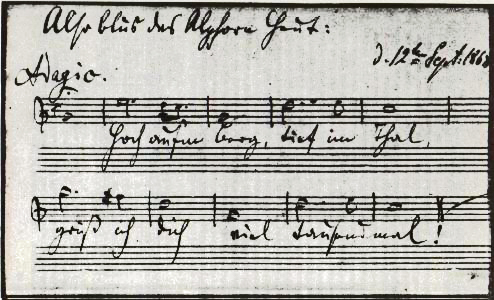
\includegraphics[clip,width=7.0cm]{./figure/alphorn.jpg}
	\caption{1868年9月, JohannesからClaraへの手紙.}
    \label{fig: alphorn}
	\end{center}
\end{figure}

1873年夏に完成したハイドンの主題による変奏曲, その年の暮れから74年頭の間に完成したピアノ四重奏曲第3番の経験を経て, Brahmsはハ短調の交響曲を完成させる気は熟したと判断したと思われる.
Simrockに「交響曲について心配は無用です. それはいずれ, われわれの出版社の名前で出されなければならないのですから」と手紙で伝える\cite{ogt}と,
%** この手紙の出典および書かれた時期を調べること もしかして76年だったりしない? \cite{library} **
1874年夏にスイスのリュシュリコンで第4楽章に取り組んでいる.
1875年の夏はツィーゲルハウゼンで弦楽四重奏曲第3番作品67を仕上げた\cite{compos}後に, 1876年夏のザースニッツ滞在,
そして続くバーデン・バーデン滞在中に本作に取り組み, 最終的にこの年の秋にClaraのいるリヒテンタールでの滞在中に書き上げられた (図\ref{fig: mov4-59}).
Brahmsは1876年9月に第1, 4楽章を, 10月10日には全楽章をClaraにピアノで聴かせている.
ClaraはJoachimへの手紙でこの曲を「才気に富んだ労作です」と高く評価しているものの, 旋律の活気に欠けているために「私は悲しみ,
打ちひしがれたことを隠すことができません」とも同じ手紙で述べている\cite{compos}.


\section{初演と評価}\label{sec: premiere}

Brahmsは指揮者Otto Dessoffに楽譜を見せ, その意見をもとに改訂を加えつつ, 初演の準備を進めた.
初演は1876年11月4日, Dessoffの指揮, カールスルーエ宮廷管弦楽団の第1回予約演奏会で行われた.
それに先立つ8月13日にはバイロイト音楽祭でWagnerの「ニーベルングの指環」が初演されていることと比較すると, 優れて象徴的である.
初演の後, 半年かけてBrahmsは本作を手稿譜のまま携えて演奏旅行に出かけた (詳細な演奏データは\ref{sec: till publication}節参照).
この過程は自作の紹介とともに出版前に作品を改訂するためのもので, Brahmsはどの交響曲についてもこのプロセスを必ず綿密に遂行している.
Brahmsは常に出版稿に至るまでの途中段階の楽譜を破棄しているが, この曲に関しては,
この「試演」段階で使用されたVn1, Vn2, Vaのパート譜が完全には破棄されずに残されており, 初演時と出版時でどのような変更が加えらえたのかを窺い知ることができる.
それによると, 第2楽章は初演時には現在よりもずっと大規模で, A+B+A+C+Aという構造を取っていた.
初演稿はHenle社のスタディスコアの付録として見ることができる\cite{henle}し, Riccardo Chailly/ライプツィヒ・ゲヴァントハウス管弦楽団の2012-13年の録音などで聴くこともできる.

交響曲史上でも傑出した本作であるが, 初演および一連の演奏は賛否両論の激しい議論を引き起こし, (ハンブルクでの演奏を除き) 大成功と言えるものではなかった\cite{compos}.
特にウィーンでは演奏後に拍手が起こらなかったと伝えられる (回想録集\cite{kaisouroku}第2巻p.22-23).
これはもちろん作品自体が複雑で一聴しただけで十分に理解するのが難しいという点にも要因があるが, 何より\ref{sec: premiere}節で論じた「Beethoven問題」が大きく寄与している:
当時の評論家の問題意識は「Brahmsの新作の交響曲はBeethovenの交響曲の伝統のもとでどのように位置づけるべきか」という点に向けられていた\cite{frisch}.

coming soon


\section{出版}

完成版の楽譜がBrahmsからSimrockに発送されたのは1877年5月31日 (第2楽章を除く) で\cite{library},
1877年10月に管弦楽版総譜, パート譜, ピアノ連弾版が同時に出版されている\cite{frisch}. 出版報酬は5000ターラーであった\cite{henle}.
出版の遅れは同じ時期に交響曲第2番の作曲が進められていたことが影響していると考えられる.

出版用のスコア自筆譜は1楽章のみ1900年代初頭に失われているが, 2, 3, 4楽章はピアーポント・モーガン図書館に収蔵されている.
4楽章の終わりに"J.~Brahms Lichtenthal Sept: 76"と書き込まれている (図\ref{fig: mov4-59}) が, 当然その第2楽章はそれ以後に作成されたものである.
ピアノ連弾版自筆譜はアメリカ議会図書館に収蔵されていて, "Pörtschach Juni 77. J.~Br."と署名されている\cite{frisch}.

現在普及している楽譜は, 他の交響曲もそうだが, 1920年代のBreitkopf \& Härtel社によるBrahms全集を底本としている.
この全集版にはEusebius Mandyczewskiも加わっているが, 特に器楽曲に関してはHans Gálが編集主幹として作業に当たっている.
Dover版, あるいは国内版である音楽之友社版\cite{ogt}, 全音版はいずれもこの流れに位置づけられる.

ただ, このBH全集版は自筆譜ではなく, ウィーン楽友協会に保管されている作曲者の書き込み付き初版譜をもとにしている.
この書き込みには一時的な試し書きも含まれており, どれだけBrahmsの最終的な決定を反映しているかが微妙な問題である.
この点に注意を払ったRobert Pascall校訂による新版がHenle社から1997年に出版されている\cite{henle}.
ただしこの曲に関してはHenle版とBH全集版とでさほど重大な相違は見られない.
% むしろこの新版には破棄を免れたカールスルーエ初演時の1st, 2ndヴァイオリンとヴィオラのパート譜が付録として掲載されていることが興味深い.

なお, \href{http://imslp.org/wiki/Symphony_No.1,_Op.68_(Brahms,_Johannes)}{IMSLP}から,
管弦楽版自筆譜 (1楽章を除く), ピアノ連弾版自筆譜, Simrock社の管弦楽版初版譜, BH全集版初版譜, BH全集版パート譜などがダウンロードできる.

\begin{figure}[htbp]
	\centering
    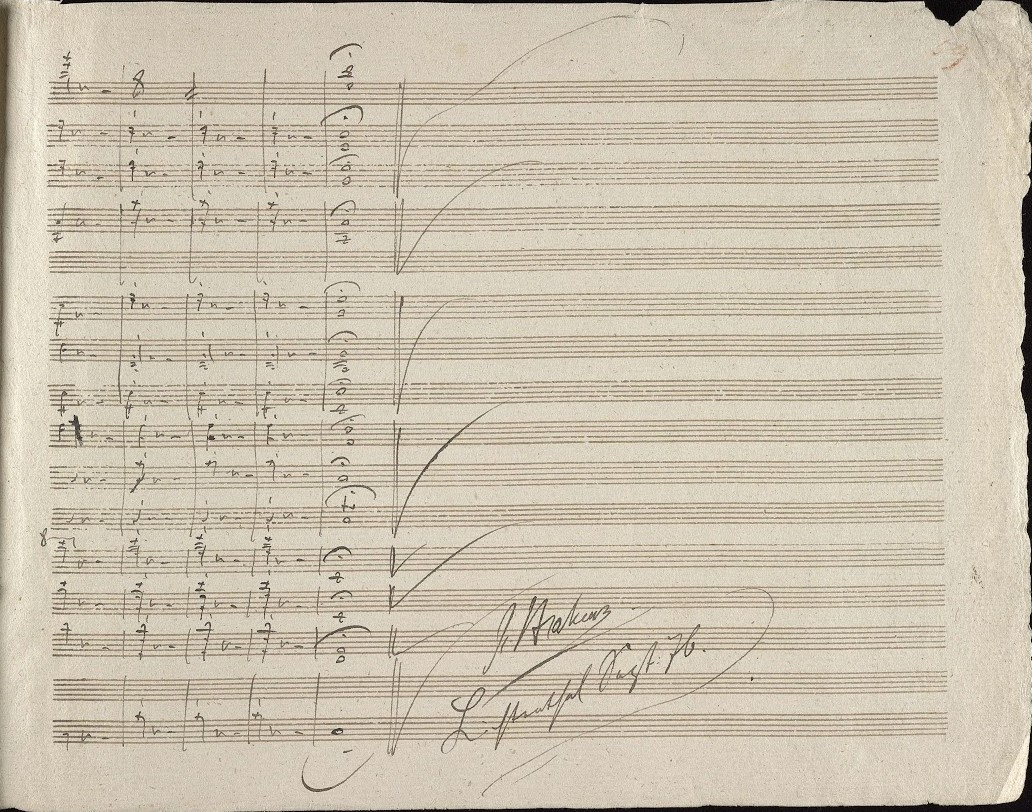
\includegraphics[clip,width=12.0cm]{./figure/mov4-59.jpg}
	\caption{自筆譜の最終ページ}
    \label{fig: mov4-59}
\end{figure}

\begin{figure}[htbp]
	\centering
    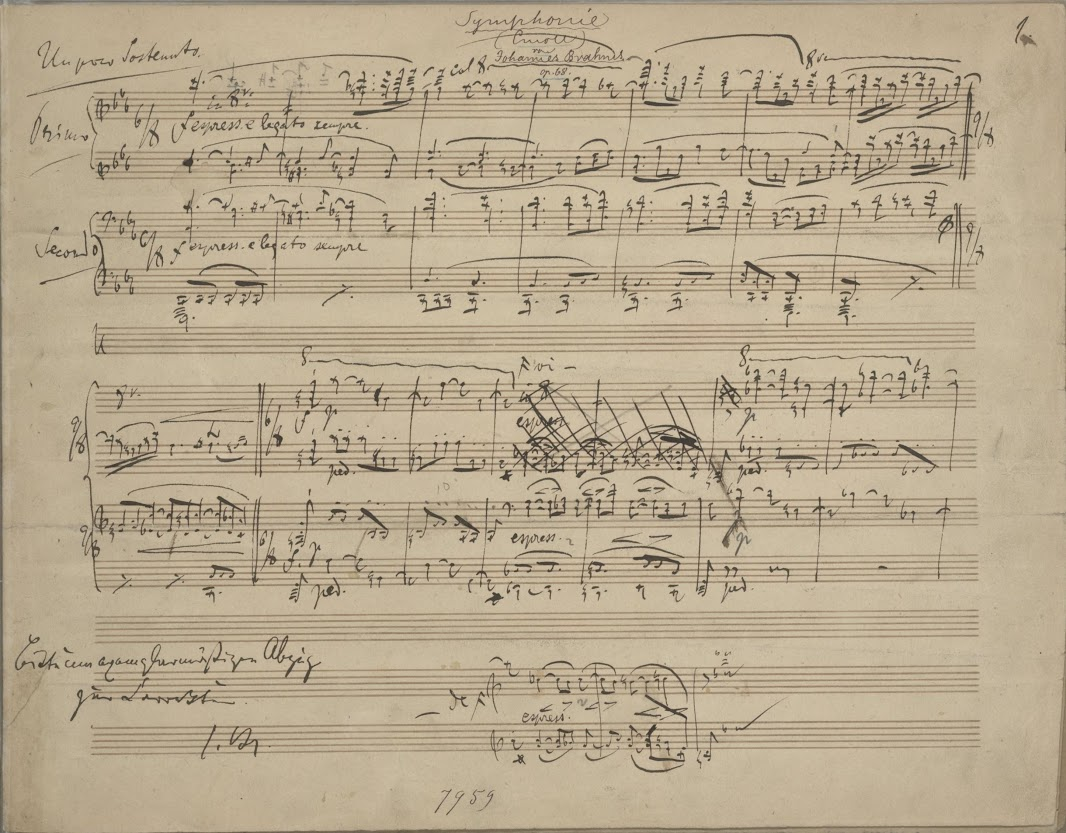
\includegraphics[clip,width=12.0cm]{./figure/mov1(4H)-01.jpg}
	\caption{ピアノ連弾版自筆譜の冒頭ページ}
    \label{fig: mov1(4H)-01}
\end{figure}
